%%%%%%%%%%%%%%%%%%%%%%%%%%%%%%%%%%%%%%%%%
% Journal Article
% LaTeX Template
% Version 1.3 (9/9/13)
%
% This template has been downloaded from:
% http://www.LaTeXTemplates.com
%
% Original author:
% Frits Wenneker (http://www.howtotex.com)
%
% License:
% CC BY-NC-SA 3.0 (http://creativecommons.org/licenses/by-nc-sa/3.0/)
%
%%%%%%%%%%%%%%%%%%%%%%%%%%%%%%%%%%%%%%%%%

%----------------------------------------------------------------------------------------
%	PACKAGES AND OTHER DOCUMENT CONFIGURATIONS
%----------------------------------------------------------------------------------------

\documentclass[twoside]{article}

\usepackage{lipsum} % Package to generate dummy text throughout this template

\usepackage{graphicx}

%\usepackage[portuguese]{babel}
%\usepackage[latin1]{inputenc} 

\usepackage[sc]{mathpazo} % Use the Palatino font
\usepackage[utf8]{inputenc} %%o milagre que deu conta dos acentos, aparentemente.
%\usepackage[T1]{fontenc} % Use 8-bit encoding that has 256 glyphs
\linespread{1.05} % Line spacing - Palatino needs more space between lines
\usepackage{microtype} % Slightly tweak font spacing for aesthetics

\usepackage[hmarginratio=1:1,top=32mm,columnsep=20pt]{geometry} % Document margins
\usepackage{multicol} % Used for the two-column layout of the document
\usepackage[hang, small,labelfont=bf,up,textfont=it,up]{caption} % Custom captions under/above floats in tables or figures
\usepackage{booktabs} % Horizontal rules in tables
\usepackage{float} % Required for tables and figures in the multi-column environment - they need to be placed in specific locations with the [H] (e.g. \begin{table}[H])
\usepackage{hyperref} % For hyperlinks in the PDF

\usepackage{lettrine} % The lettrine is the first enlarged letter at the beginning of the text
\usepackage{paralist} % Used for the compactitem environment which makes bullet points with less space between them

\usepackage{abstract} % Allows abstract customization
\renewcommand{\abstractnamefont}{\normalfont\bfseries} % Set the "Abstract" text to bold
\renewcommand{\abstracttextfont}{\normalfont\small\itshape} % Set the abstract itself to small italic text

\usepackage{titlesec} % Allows customization of titles
\renewcommand\thesection{\Roman{section}} % Roman numerals for the sections
\renewcommand\thesubsection{\Roman{subsection}} % Roman numerals for subsections
\titleformat{\section}[block]{\large\scshape\centering}{\thesection.}{1em}{} % Change the look of the section titles
\titleformat{\subsection}[block]{\large}{\thesubsection.}{1em}{} % Change the look of the section titles

\usepackage{fancyhdr} % Headers and footers
\pagestyle{fancy} % All pages have headers and footers
\fancyhead{} % Blank out the default header
\fancyfoot{} % Blank out the default footer
\fancyhead[C]{PVC - Sombras $\bullet$ setembro de 2013} % Custom header text
\fancyfoot[RO,LE]{\thepage} % Custom footer text

%----------------------------------------------------------------------------------------
%	TITLE SECTION
%----------------------------------------------------------------------------------------

\title{\vspace{-15mm}\fontsize{24pt}{10pt}\selectfont\textbf{Projeto Demonstrativo 01 - Detecção de Sombras}} % Article title

\author{
\large
\textsc{Eduardo Furtado - 090111575}\thanks{-}\\[2mm] % Your name
\normalsize Princípios de Visão Computacional – Turma A - 2/2013 \\ % Your institution
\normalsize \href{mailto:eduardoxfurtado@gmail.com}{eduardoxfurtado@gmail.com} % Your email address
\vspace{-5mm}
}
\date{}

%----------------------------------------------------------------------------------------

\begin{document}

\maketitle % Insert title

\thispagestyle{fancy} % All pages have headers and footers

%----------------------------------------------------------------------------------------
%	ABSTRACT
%----------------------------------------------------------------------------------------

\begin{abstract}

\noindent %%\lipsum[1] % Dummy abstract text
Desenvolvimento de técnicas simples para auxílio na remoção de sombras em vídeo e utilização da Biblioteca de Visão Computacional OpenCV.


\end{abstract}

%----------------------------------------------------------------------------------------
%	ARTICLE CONTENTS
%----------------------------------------------------------------------------------------

\begin{multicols}{2} % Two-column layout throughout the main article text

\section{Introdução}

\lettrine[nindent=0em,lines=2]{I} nspirado na metodologia do artigo científico de Stauder,1999 - "Shadows removal", e utilizou-se também as ténicas propostas na descrição do trabalho para remoção de fundo, histograma e separação da sombra.
%\lipsum[2-3] % Dummy text

%------------------------------------------------

\section{Materiais}

 
Inicialmente tentou-se configurar o ambiente para a plataforma windows.\\
Por fim optou-se pelo Linux Mint 14, devido a facilidade da instalação do OpenCV 2.3. \\
O G++ (Ubuntu/Linaro 4.7.2-2ubuntu1) foi o compilador C++ utilizado. A seguinda linha foi usada:\\
g++ 090111575.cpp -o 090111575 `pkg-config --cflags --libs opencv`;
\\Vídeo 'highwayI\_raw.avi' fornecido na descrição da tarefa.
\\Para este documento foi utilizado o writelatex, programa disponível online.

%------------------------------------------------

\section{Métodos}
Após horas perdidas em tentativas frustradas, a passos lentos e curtos, na plataforma Windows, recomeçei o trabalho no ambiente Unix. 
\\Pintei as sombras em cada um dos frames de um vídeo. Para isso utilizei uma técnica para separar o fundo (background) de cada frame (utilizando os 2 frames anteriores, n=2). Calculei um histograma dos valores de negro dos pixels que não faziam parte do fundo, e baseando-me neste histograma, pintei os pixels mais escuros da cor verde. Os pixels restantes permaneceram inalterados. O valor do limiar do pixel para a cor negra é escolhido a cada frame, baseando-se no histograma. O cálculo é feito supongo que metade dos pixels que não são parte do fundo devem ser pixels de sombra e eles são os mais próximos do negro.
\\Para separar o fundo, utilizou-se um valor de limiar de 25, ou seja, pixels que diferiam em 25 entre um frame e outro, eram considerados diferentes, e portanto pertenciam a objetos em movimento e não ao fundo.
\\O histograma feito dividia os 256 valores possíveis a um pixel em 16 grupos de 16 valores.
\\Finalmente as sombras foram pintadas de verde, segundo o padrão RGB: 0-255-0.
\\Os vídeos são todos mostrados em tempo real, em janelas que abrem próximas umas as outras, com a mesma taxa de frames, que pode ser alterada no código com a constante velocidade\_reproducao.



%\begin{compactitem}
%\item Donec dolor arcu, rutrum id molestie in, viverra sed diam
%\item Curabitur feugiat
%\item turpis sed auctor facilisis
%\item arcu eros accumsan lorem, at posuere mi diam sit amet tortor
%\item Fusce fermentum, mi sit amet euismod rutrum
%\item sem lorem molestie diam, iaculis aliquet sapien tortor non nisi
%\item Pellentesque bibendum pretium aliquet
%\end{compactitem}

%------------------------------------------------

\section{Resultados}

\begin{figure}[H]
\centering
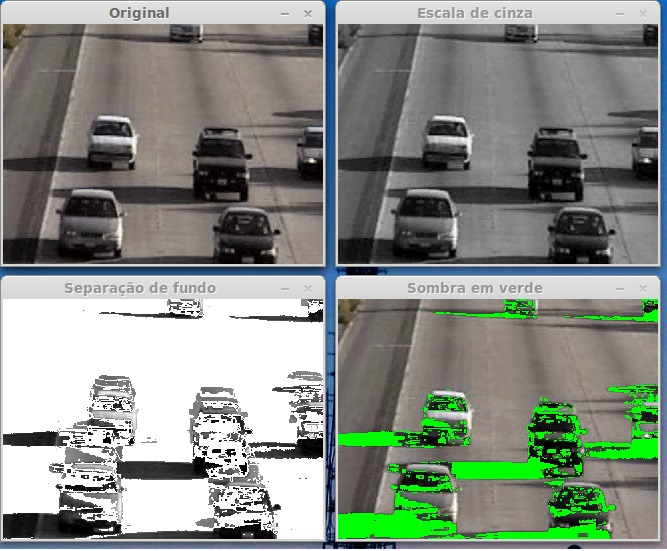
\includegraphics[width=75mm]{resultados.jpg}
\caption{Imagem do vídeo original e dos resultados obtidos}
\label{overflow}
\end{figure}

A imagem acima é um exelente exemplo do que foi alcançado utilizando os parametros que geraram melhor resultado. Para a separação do fundo foi usado 25 como valor de limiar, baseado na observação do que gerava melhores resultados.\\Da mesma maneira a opção de dividir os objetos em 2 grupos de pixels: metade deveria ser o objeto e a outra metade a sombra desse objeto.

%\begin{table}[H]
%\caption{Example table}
%\centering
%\begin{tabular}{llr}
%\toprule
%\multicolumn{2}{c}{Name} \\
%\cmidrule(r){1-2}
%First name & Last Name & Grade \\
%\midrule
%John & Doe & $7.5$ \\
%Richard & Miles & $2$ \\
%\bottomrule
%\end{tabular}
%\end{table}


%\begin{equation}
%\label{eq:emc}
%e = mc^2
%\end{equation}


%------------------------------------------------

\section{Discussão e conclusão}

Os resultados obtidos foram satisfatórios, entretanto não foram perfeitos. Conseguiu-se separar a sombra, entretanto há margem para melhoria, tendo em vista que a separação do que é um objeto e o que é a sombra desse objeto nem sempre é perfeita. Mesmo assim isso é algo a ser argumentado, já que como os objetos alvo eram carros, coisas grandes, eles mesmo fazem sombra neles mesmo: o teto do carro faz sombra, de fato, no painel de controle do carro ou mesmo sobre o rosto do motorista.\\
Outro aspecto a ser discutido é se sombras de objetos estáticos devem ser consideradas fundo ou não. No caso, foram consideradas fundo.
\\Objetos extremamente grades apontam para falhar no algoritmo, provavelmente devido ao fato de serem tão grandes a ponto de confundirem-se com o fundo. A correção desse problema poderia ser feita tomando n>>2, por exemplo n=50 como proposto no artigo de segmentação do fundo.

%\subsection{Subsection One}

%\lipsum[7] % Dummy text

%\subsection{Subsection Two}

%\lipsum[8] % Dummy text

%----------------------------------------------------------------------------------------
%	REFERENCE LIST
%----------------------------------------------------------------------------------------

\begin{thebibliography}{99} % Bibliography - this is intentionally simple in this template


\bibitem{opencv} Documentação oficial do OpenCV, \emph{último acesso em 23/09/2013},  disponível em \\
\url{http://docs.opencv.org/}.

%\bibitem[Figueredo and Wolf, 2009]{Figueredo:2009dg}
%Figueredo, A.~J. and Wolf, P. S.~A. (2009).
%\newblock Assortative pairing and life history strategy - a cross-cultural
%  study.
%\newblock {\em Human Nature}, 20:317--330.



 
\end{thebibliography}

%----------------------------------------------------------------------------------------

\end{multicols}

\end{document}